\PassOptionsToPackage{unicode=true}{hyperref} % options for packages loaded elsewhere
\PassOptionsToPackage{hyphens}{url}
%
\documentclass[]{article}
\usepackage{lmodern}
\usepackage{amssymb,amsmath}
\usepackage{ifxetex,ifluatex}
\usepackage{fixltx2e} % provides \textsubscript
\ifnum 0\ifxetex 1\fi\ifluatex 1\fi=0 % if pdftex
  \usepackage[T1]{fontenc}
  \usepackage[utf8]{inputenc}
  \usepackage{textcomp} % provides euro and other symbols
\else % if luatex or xelatex
  \usepackage{unicode-math}
  \defaultfontfeatures{Ligatures=TeX,Scale=MatchLowercase}
\fi
% use upquote if available, for straight quotes in verbatim environments
\IfFileExists{upquote.sty}{\usepackage{upquote}}{}
% use microtype if available
\IfFileExists{microtype.sty}{%
\usepackage[]{microtype}
\UseMicrotypeSet[protrusion]{basicmath} % disable protrusion for tt fonts
}{}
\IfFileExists{parskip.sty}{%
\usepackage{parskip}
}{% else
\setlength{\parindent}{0pt}
\setlength{\parskip}{6pt plus 2pt minus 1pt}
}
\usepackage{hyperref}
\hypersetup{
            pdftitle={Homework Q6},
            pdfauthor={Gayatri Mainkar},
            pdfborder={0 0 0},
            breaklinks=true}
\urlstyle{same}  % don't use monospace font for urls
\usepackage[margin=1in]{geometry}
\usepackage{color}
\usepackage{fancyvrb}
\newcommand{\VerbBar}{|}
\newcommand{\VERB}{\Verb[commandchars=\\\{\}]}
\DefineVerbatimEnvironment{Highlighting}{Verbatim}{commandchars=\\\{\}}
% Add ',fontsize=\small' for more characters per line
\usepackage{framed}
\definecolor{shadecolor}{RGB}{248,248,248}
\newenvironment{Shaded}{\begin{snugshade}}{\end{snugshade}}
\newcommand{\AlertTok}[1]{\textcolor[rgb]{0.94,0.16,0.16}{#1}}
\newcommand{\AnnotationTok}[1]{\textcolor[rgb]{0.56,0.35,0.01}{\textbf{\textit{#1}}}}
\newcommand{\AttributeTok}[1]{\textcolor[rgb]{0.77,0.63,0.00}{#1}}
\newcommand{\BaseNTok}[1]{\textcolor[rgb]{0.00,0.00,0.81}{#1}}
\newcommand{\BuiltInTok}[1]{#1}
\newcommand{\CharTok}[1]{\textcolor[rgb]{0.31,0.60,0.02}{#1}}
\newcommand{\CommentTok}[1]{\textcolor[rgb]{0.56,0.35,0.01}{\textit{#1}}}
\newcommand{\CommentVarTok}[1]{\textcolor[rgb]{0.56,0.35,0.01}{\textbf{\textit{#1}}}}
\newcommand{\ConstantTok}[1]{\textcolor[rgb]{0.00,0.00,0.00}{#1}}
\newcommand{\ControlFlowTok}[1]{\textcolor[rgb]{0.13,0.29,0.53}{\textbf{#1}}}
\newcommand{\DataTypeTok}[1]{\textcolor[rgb]{0.13,0.29,0.53}{#1}}
\newcommand{\DecValTok}[1]{\textcolor[rgb]{0.00,0.00,0.81}{#1}}
\newcommand{\DocumentationTok}[1]{\textcolor[rgb]{0.56,0.35,0.01}{\textbf{\textit{#1}}}}
\newcommand{\ErrorTok}[1]{\textcolor[rgb]{0.64,0.00,0.00}{\textbf{#1}}}
\newcommand{\ExtensionTok}[1]{#1}
\newcommand{\FloatTok}[1]{\textcolor[rgb]{0.00,0.00,0.81}{#1}}
\newcommand{\FunctionTok}[1]{\textcolor[rgb]{0.00,0.00,0.00}{#1}}
\newcommand{\ImportTok}[1]{#1}
\newcommand{\InformationTok}[1]{\textcolor[rgb]{0.56,0.35,0.01}{\textbf{\textit{#1}}}}
\newcommand{\KeywordTok}[1]{\textcolor[rgb]{0.13,0.29,0.53}{\textbf{#1}}}
\newcommand{\NormalTok}[1]{#1}
\newcommand{\OperatorTok}[1]{\textcolor[rgb]{0.81,0.36,0.00}{\textbf{#1}}}
\newcommand{\OtherTok}[1]{\textcolor[rgb]{0.56,0.35,0.01}{#1}}
\newcommand{\PreprocessorTok}[1]{\textcolor[rgb]{0.56,0.35,0.01}{\textit{#1}}}
\newcommand{\RegionMarkerTok}[1]{#1}
\newcommand{\SpecialCharTok}[1]{\textcolor[rgb]{0.00,0.00,0.00}{#1}}
\newcommand{\SpecialStringTok}[1]{\textcolor[rgb]{0.31,0.60,0.02}{#1}}
\newcommand{\StringTok}[1]{\textcolor[rgb]{0.31,0.60,0.02}{#1}}
\newcommand{\VariableTok}[1]{\textcolor[rgb]{0.00,0.00,0.00}{#1}}
\newcommand{\VerbatimStringTok}[1]{\textcolor[rgb]{0.31,0.60,0.02}{#1}}
\newcommand{\WarningTok}[1]{\textcolor[rgb]{0.56,0.35,0.01}{\textbf{\textit{#1}}}}
\usepackage{graphicx,grffile}
\makeatletter
\def\maxwidth{\ifdim\Gin@nat@width>\linewidth\linewidth\else\Gin@nat@width\fi}
\def\maxheight{\ifdim\Gin@nat@height>\textheight\textheight\else\Gin@nat@height\fi}
\makeatother
% Scale images if necessary, so that they will not overflow the page
% margins by default, and it is still possible to overwrite the defaults
% using explicit options in \includegraphics[width, height, ...]{}
\setkeys{Gin}{width=\maxwidth,height=\maxheight,keepaspectratio}
\setlength{\emergencystretch}{3em}  % prevent overfull lines
\providecommand{\tightlist}{%
  \setlength{\itemsep}{0pt}\setlength{\parskip}{0pt}}
\setcounter{secnumdepth}{0}
% Redefines (sub)paragraphs to behave more like sections
\ifx\paragraph\undefined\else
\let\oldparagraph\paragraph
\renewcommand{\paragraph}[1]{\oldparagraph{#1}\mbox{}}
\fi
\ifx\subparagraph\undefined\else
\let\oldsubparagraph\subparagraph
\renewcommand{\subparagraph}[1]{\oldsubparagraph{#1}\mbox{}}
\fi

% set default figure placement to htbp
\makeatletter
\def\fps@figure{htbp}
\makeatother


\title{Homework Q6}
\author{Gayatri Mainkar}
\date{1/30/2020}

\begin{document}
\maketitle

The below code chunk contains a function that analyzes protein drug
interactions by reading in any protein PDB data and outputting a plot of
the B-factor trend for the specified protein. Simply input the PDB
identifier of the protein to obtain this plot.

Input: a single element character vector containing the four letter PDB
identifier for online file access.

Output: Plot with the B-factor trend of the protein.

\begin{Shaded}
\begin{Highlighting}[]
\NormalTok{btrend <-}\StringTok{ }\ControlFlowTok{function}\NormalTok{(x)\{}
  
  \KeywordTok{library}\NormalTok{(}\StringTok{"bio3d"}\NormalTok{) }\CommentTok{#loads bio3d package}
\NormalTok{  s <-}\StringTok{ }\KeywordTok{read.pdb}\NormalTok{(x) }\CommentTok{#reads in specified protein}
  
\NormalTok{  s.chainA <-}\StringTok{ }\KeywordTok{trim.pdb}\NormalTok{(s, }\DataTypeTok{chain=}\StringTok{"A"}\NormalTok{, }\DataTypeTok{elety=}\StringTok{"CA"}\NormalTok{) }\CommentTok{#trims protein to subset of its atoms in chain A of type "CA"}
  
\NormalTok{  s.b <-}\StringTok{ }\NormalTok{s.chainA}\OperatorTok{$}\NormalTok{atom}\OperatorTok{$}\NormalTok{b }\CommentTok{#assigns vector of b-factors of each atom to variable}
  
  \KeywordTok{plotb3}\NormalTok{(s.b, }\DataTypeTok{sse=}\NormalTok{s.chainA, }\DataTypeTok{typ=}\StringTok{"l"}\NormalTok{, }\DataTypeTok{ylab=}\StringTok{"Bfactor"}\NormalTok{, }\DataTypeTok{main =}\NormalTok{ x) }\CommentTok{#plots the trend of the b-factor}
\NormalTok{\}}
\end{Highlighting}
\end{Shaded}

Test Case \#1

\begin{Shaded}
\begin{Highlighting}[]
\KeywordTok{btrend}\NormalTok{(}\StringTok{"4AKE"}\NormalTok{)}
\end{Highlighting}
\end{Shaded}

\begin{verbatim}
##   Note: Accessing on-line PDB file
\end{verbatim}

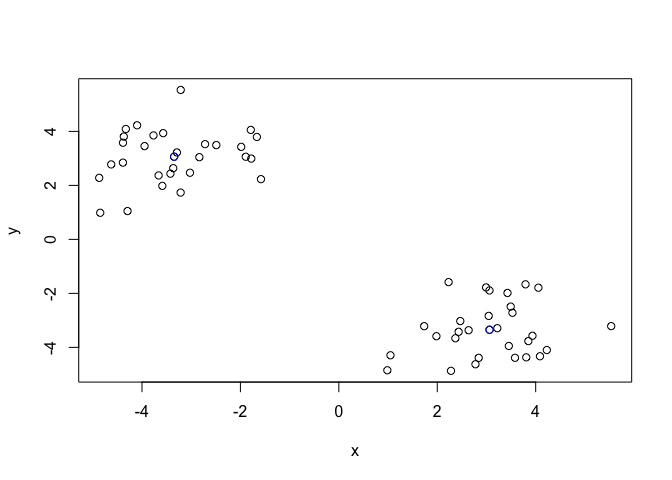
\includegraphics{HW-Q6_files/figure-latex/unnamed-chunk-2-1.pdf}

Test Case \#2

\begin{Shaded}
\begin{Highlighting}[]
\KeywordTok{btrend}\NormalTok{(}\StringTok{"1AKE"}\NormalTok{)}
\end{Highlighting}
\end{Shaded}

\begin{verbatim}
##   Note: Accessing on-line PDB file
##    PDB has ALT records, taking A only, rm.alt=TRUE
\end{verbatim}

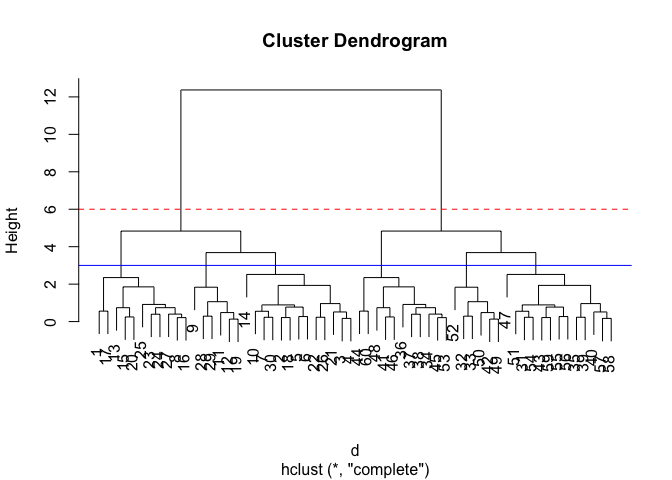
\includegraphics{HW-Q6_files/figure-latex/unnamed-chunk-3-1.pdf}

Test Case \#3

\begin{Shaded}
\begin{Highlighting}[]
\KeywordTok{btrend}\NormalTok{(}\StringTok{"1E4Y"}\NormalTok{)}
\end{Highlighting}
\end{Shaded}

\begin{verbatim}
##   Note: Accessing on-line PDB file
\end{verbatim}

\includegraphics{HW-Q6_files/figure-latex/unnamed-chunk-4-1.pdf}

\end{document}
